\documentclass[12pt,letterpaper]{article}

\usepackage{amsmath, amsthm, amsfonts, amssymb}
\usepackage{microtype, parskip, graphicx}
\usepackage[comma,numbers,sort&compress]{natbib}
\usepackage{lineno}
\usepackage{longtable}
\usepackage{docmute}
\usepackage{caption, subcaption, multirow, morefloats, rotating}
\usepackage{wrapfig}
\usepackage{hyperref}

\frenchspacing

\begin{document}

\section{Results}

\subsection{Posterior predictive results}
% why do i want to show all these graphs?
%   demonstrate how well the model recapitulates the observed data
%   if the model simulates datasets like the one we observed
%     then we can be more confident in our inferences
%   PPCs by group reveal even more about the fit of our model
%     are some time bins better predicted by others?
%     well predicted time bins indicate congruence with model assumptions
%     poorly predicted time bins indicate incongruence with model assumptions
%       something different is happening in these bins that requires explanation


% overall ppc-s
% mean
\begin{figure}[ht]
  \centering
  
\includegraphics[width=\textwidth,height=0.5\textheight,keepaspectratio=true]{figure/ppc_mean}
  \caption{<+caption text+>}
  \label{fig:<+label+>}
\end{figure}

% sd
\begin{figure}[ht]
  \centering
  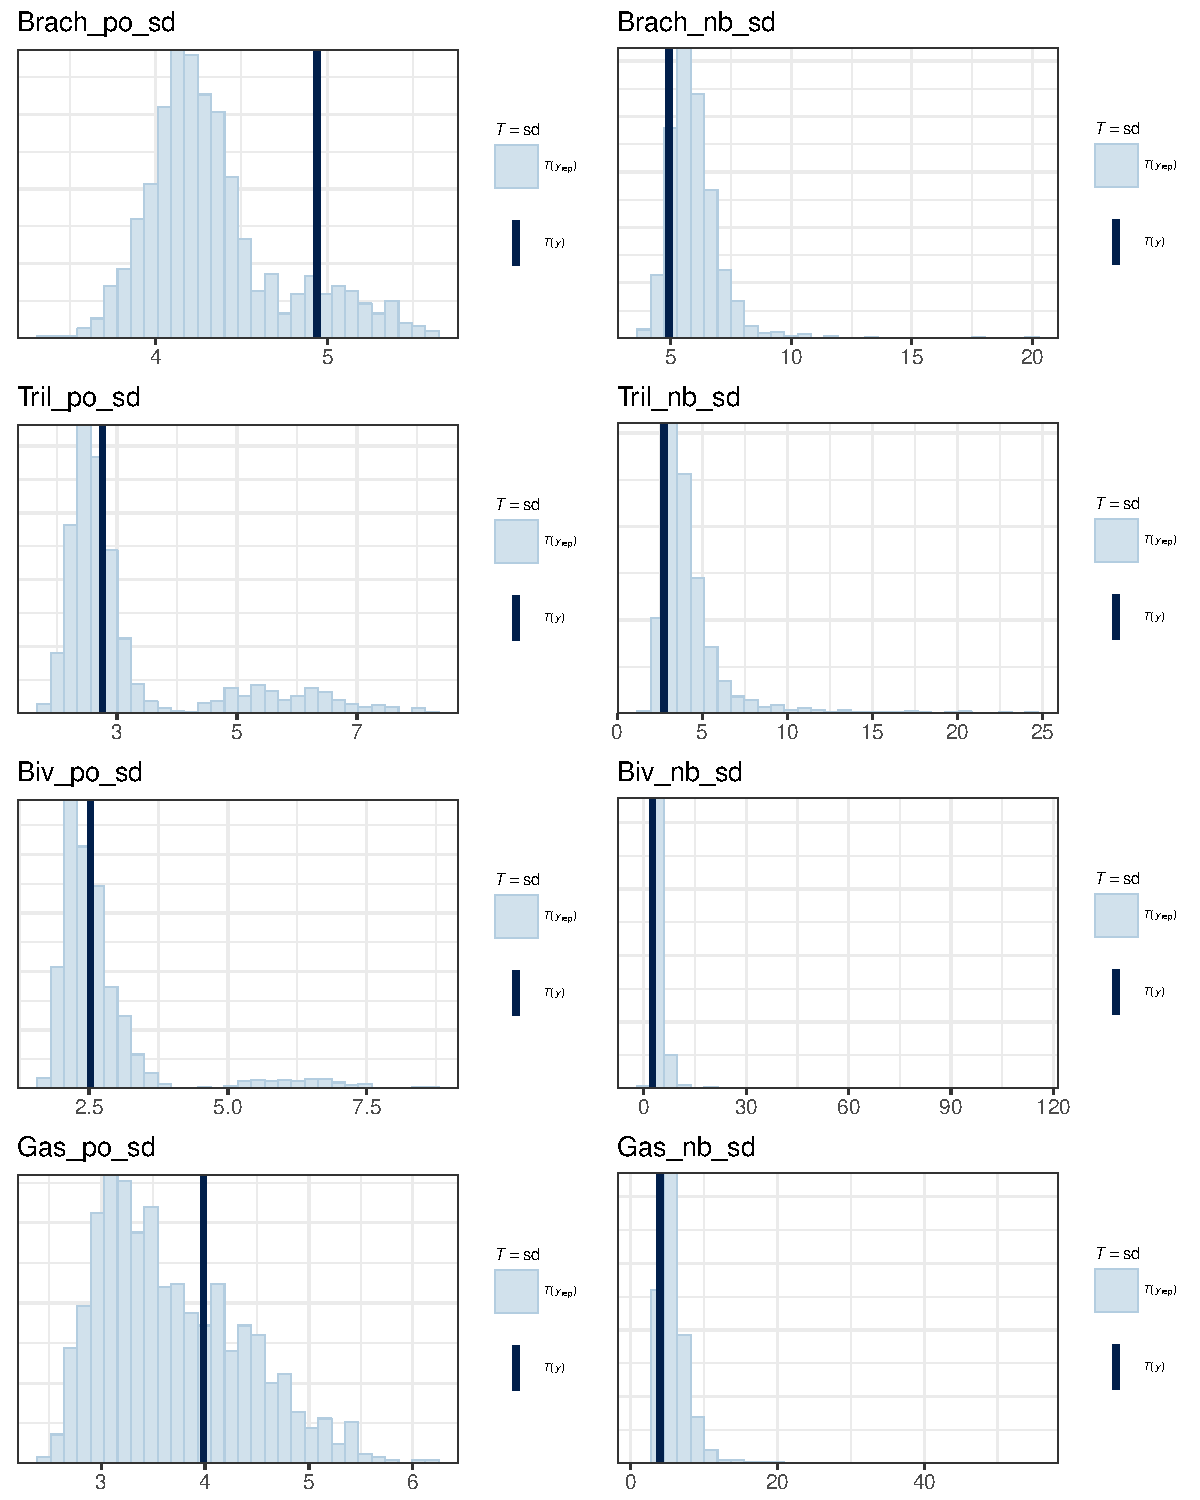
\includegraphics[width=\textwidth,height=0.5\textheight,keepaspectratio=true]{figure/ppc_sd}
  \caption{<+caption text+>}
  \label{fig:<+label+>}
\end{figure}

% ecdf
%   one of the key graphs for showing how well the distribution is mimic-d
\begin{figure}[ht]
  \centering
  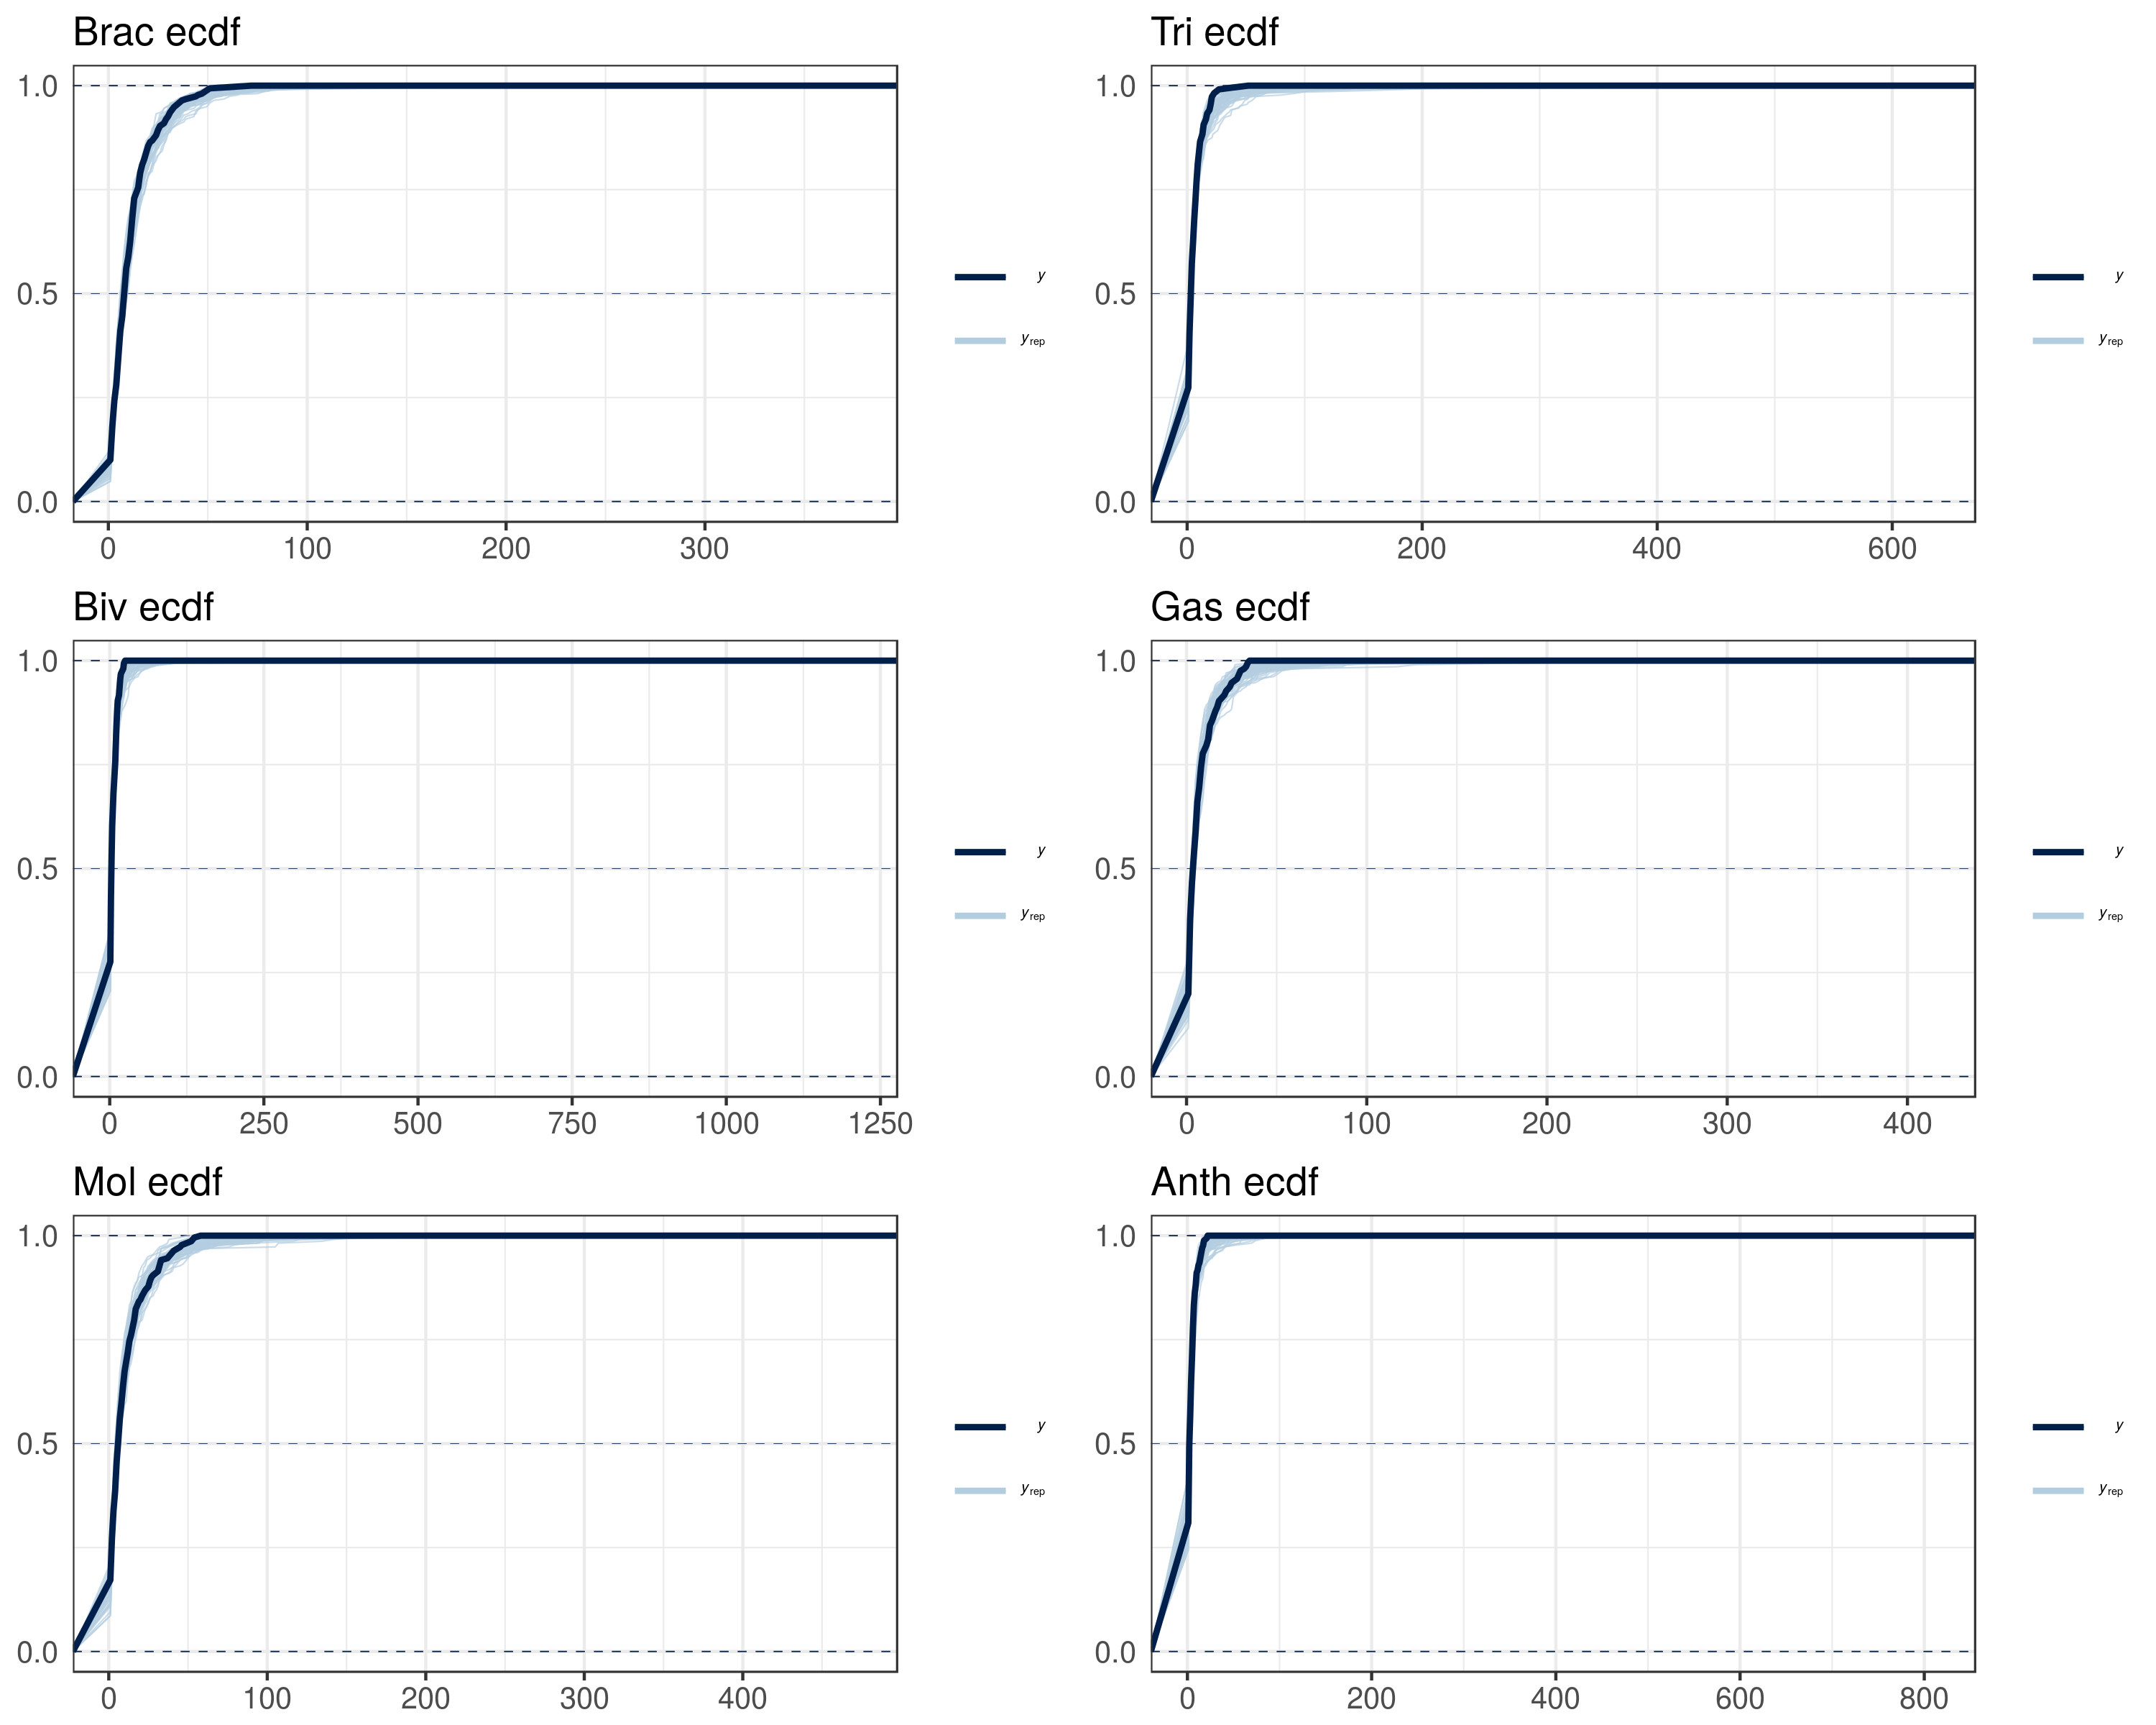
\includegraphics[width=\textwidth,height=0.5\textheight,keepaspectratio=true]{figure/ppc_ecdf}
  \caption{<+caption text+>}
  \label{fig:<+label+>}
\end{figure}

% dens
%   hard to read because size of distribution
\begin{figure}[ht]
  \centering
  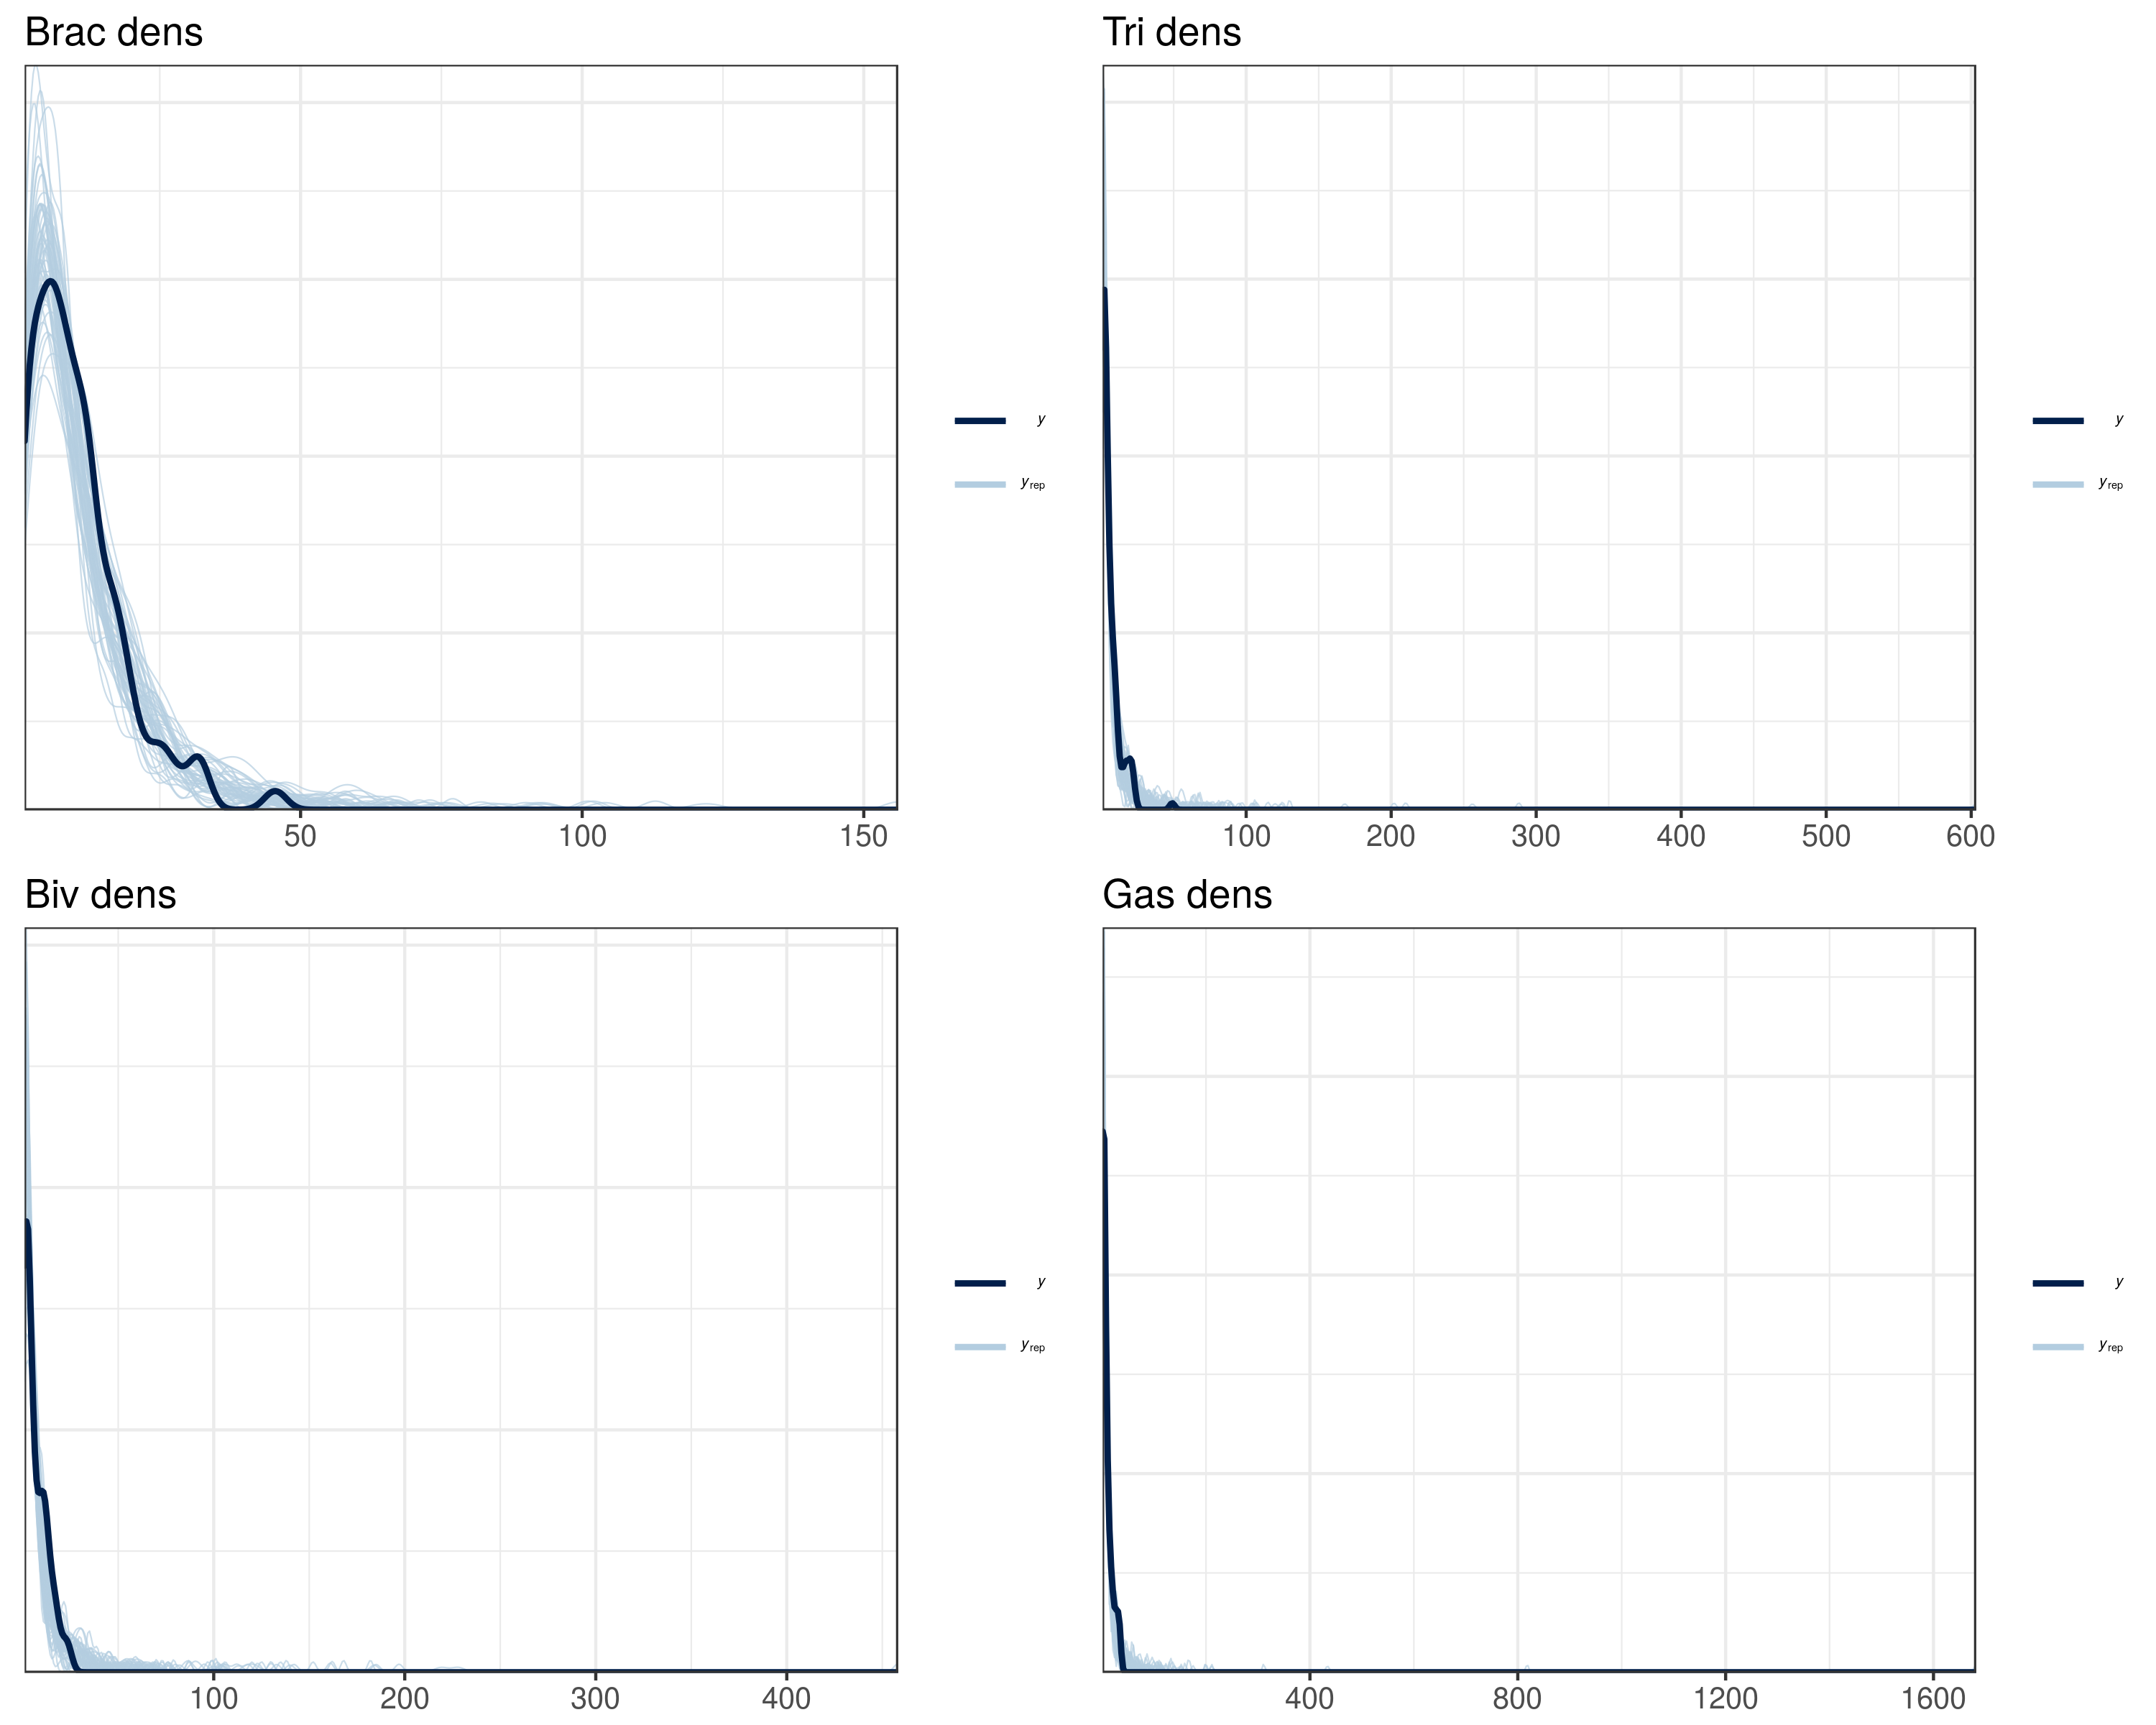
\includegraphics[width=\textwidth,height=0.5\textheight,keepaspectratio=true]{figure/ppc_dens}
  \caption{<+caption text+>}
  \label{fig:<+label+>}
\end{figure}

% dens zoomed in
%   lots of small values so need to zoom in
\begin{figure}[ht]
  \centering
  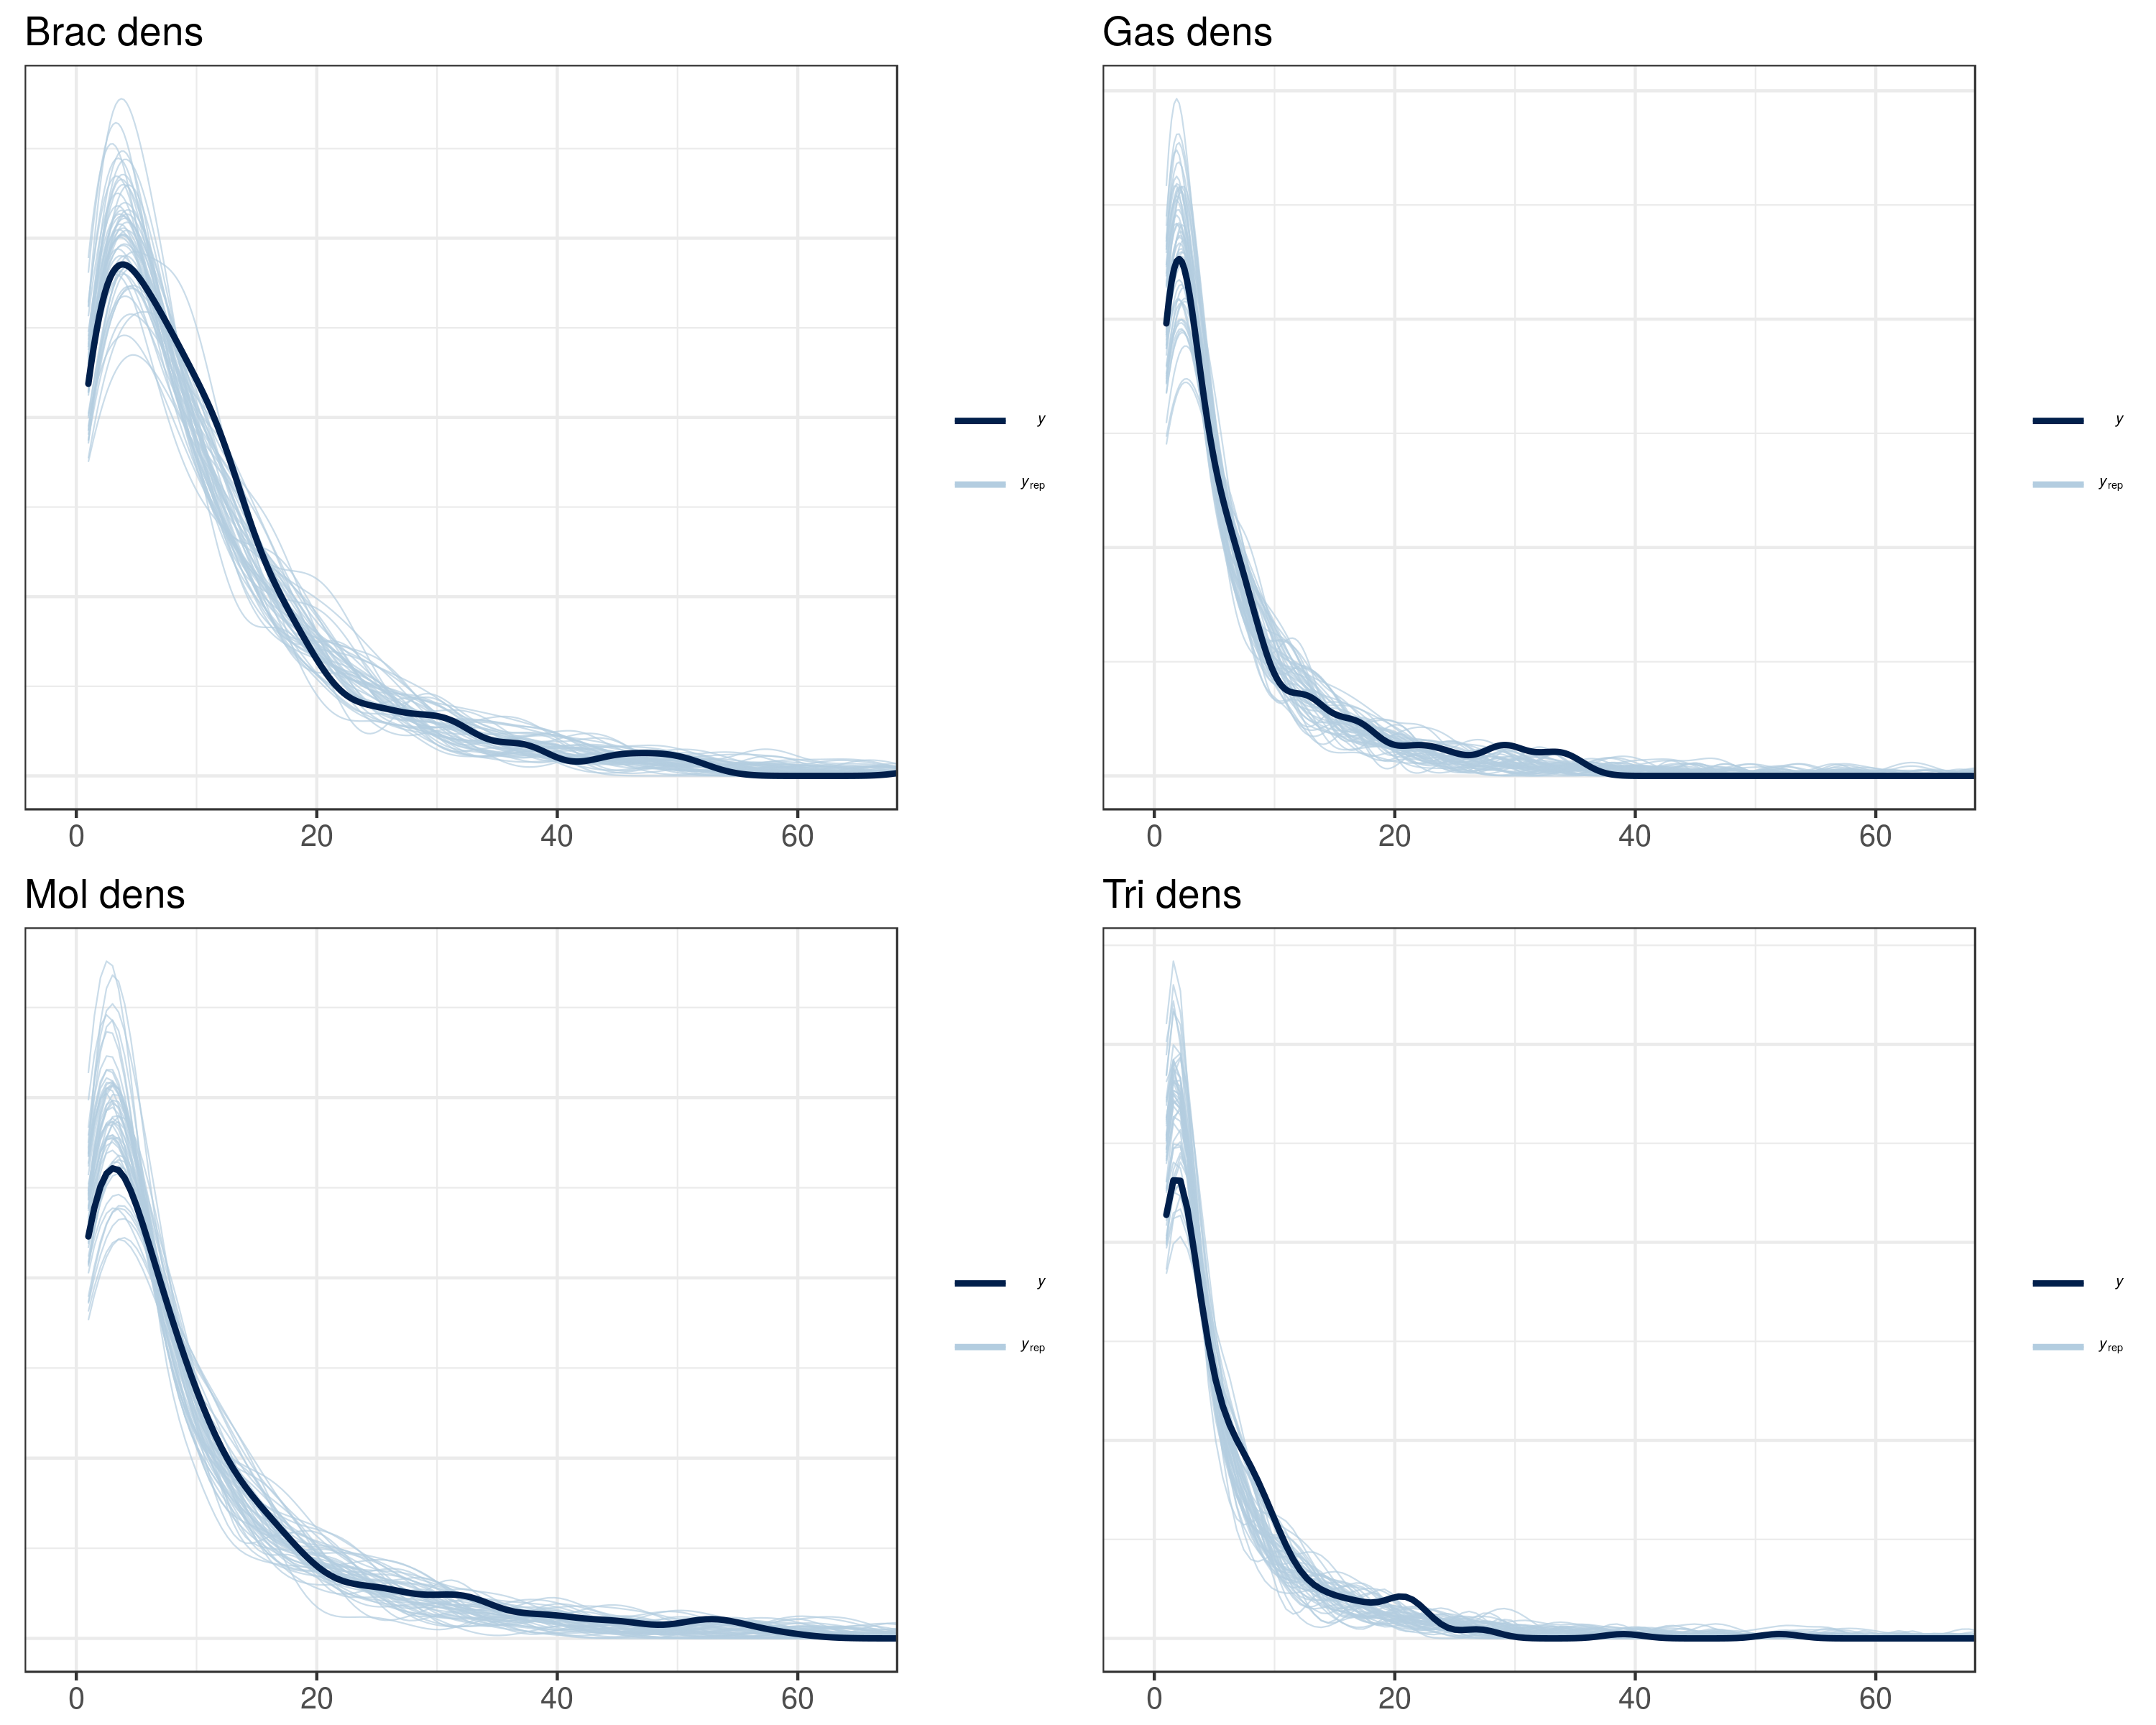
\includegraphics[width=\textwidth,height=0.5\textheight,keepaspectratio=true]{figure/ppc_dens_zoom}
  \caption{<+caption text+>}
  \label{fig:<+label+>}
\end{figure}



% group measures  
%   mean 
%     is this duplicated with my easier to read time series?
%     helps visualize the post pred skew away from empirical estimate
%   sd





\subsection{Estimated versus observed unit diversity}
% what is the point of this section?
%   graph unit diversity by time bin
%   compare to estimate from model
%   this is like the ppc for group mean, but inside-out
%   if model has poor estimates for time bin
%     that bin is not like what we would expect based on our model
%   if we have good estimates for all bins
%     then we need to look at covariates to see if there are any switch patterns


% time series graph
% what does this graph represent?
%   geological unit diversity counts at time bins
%   comparison to posterior predictive mean est with 80CI
\begin{figure}[ht]
  \centering
  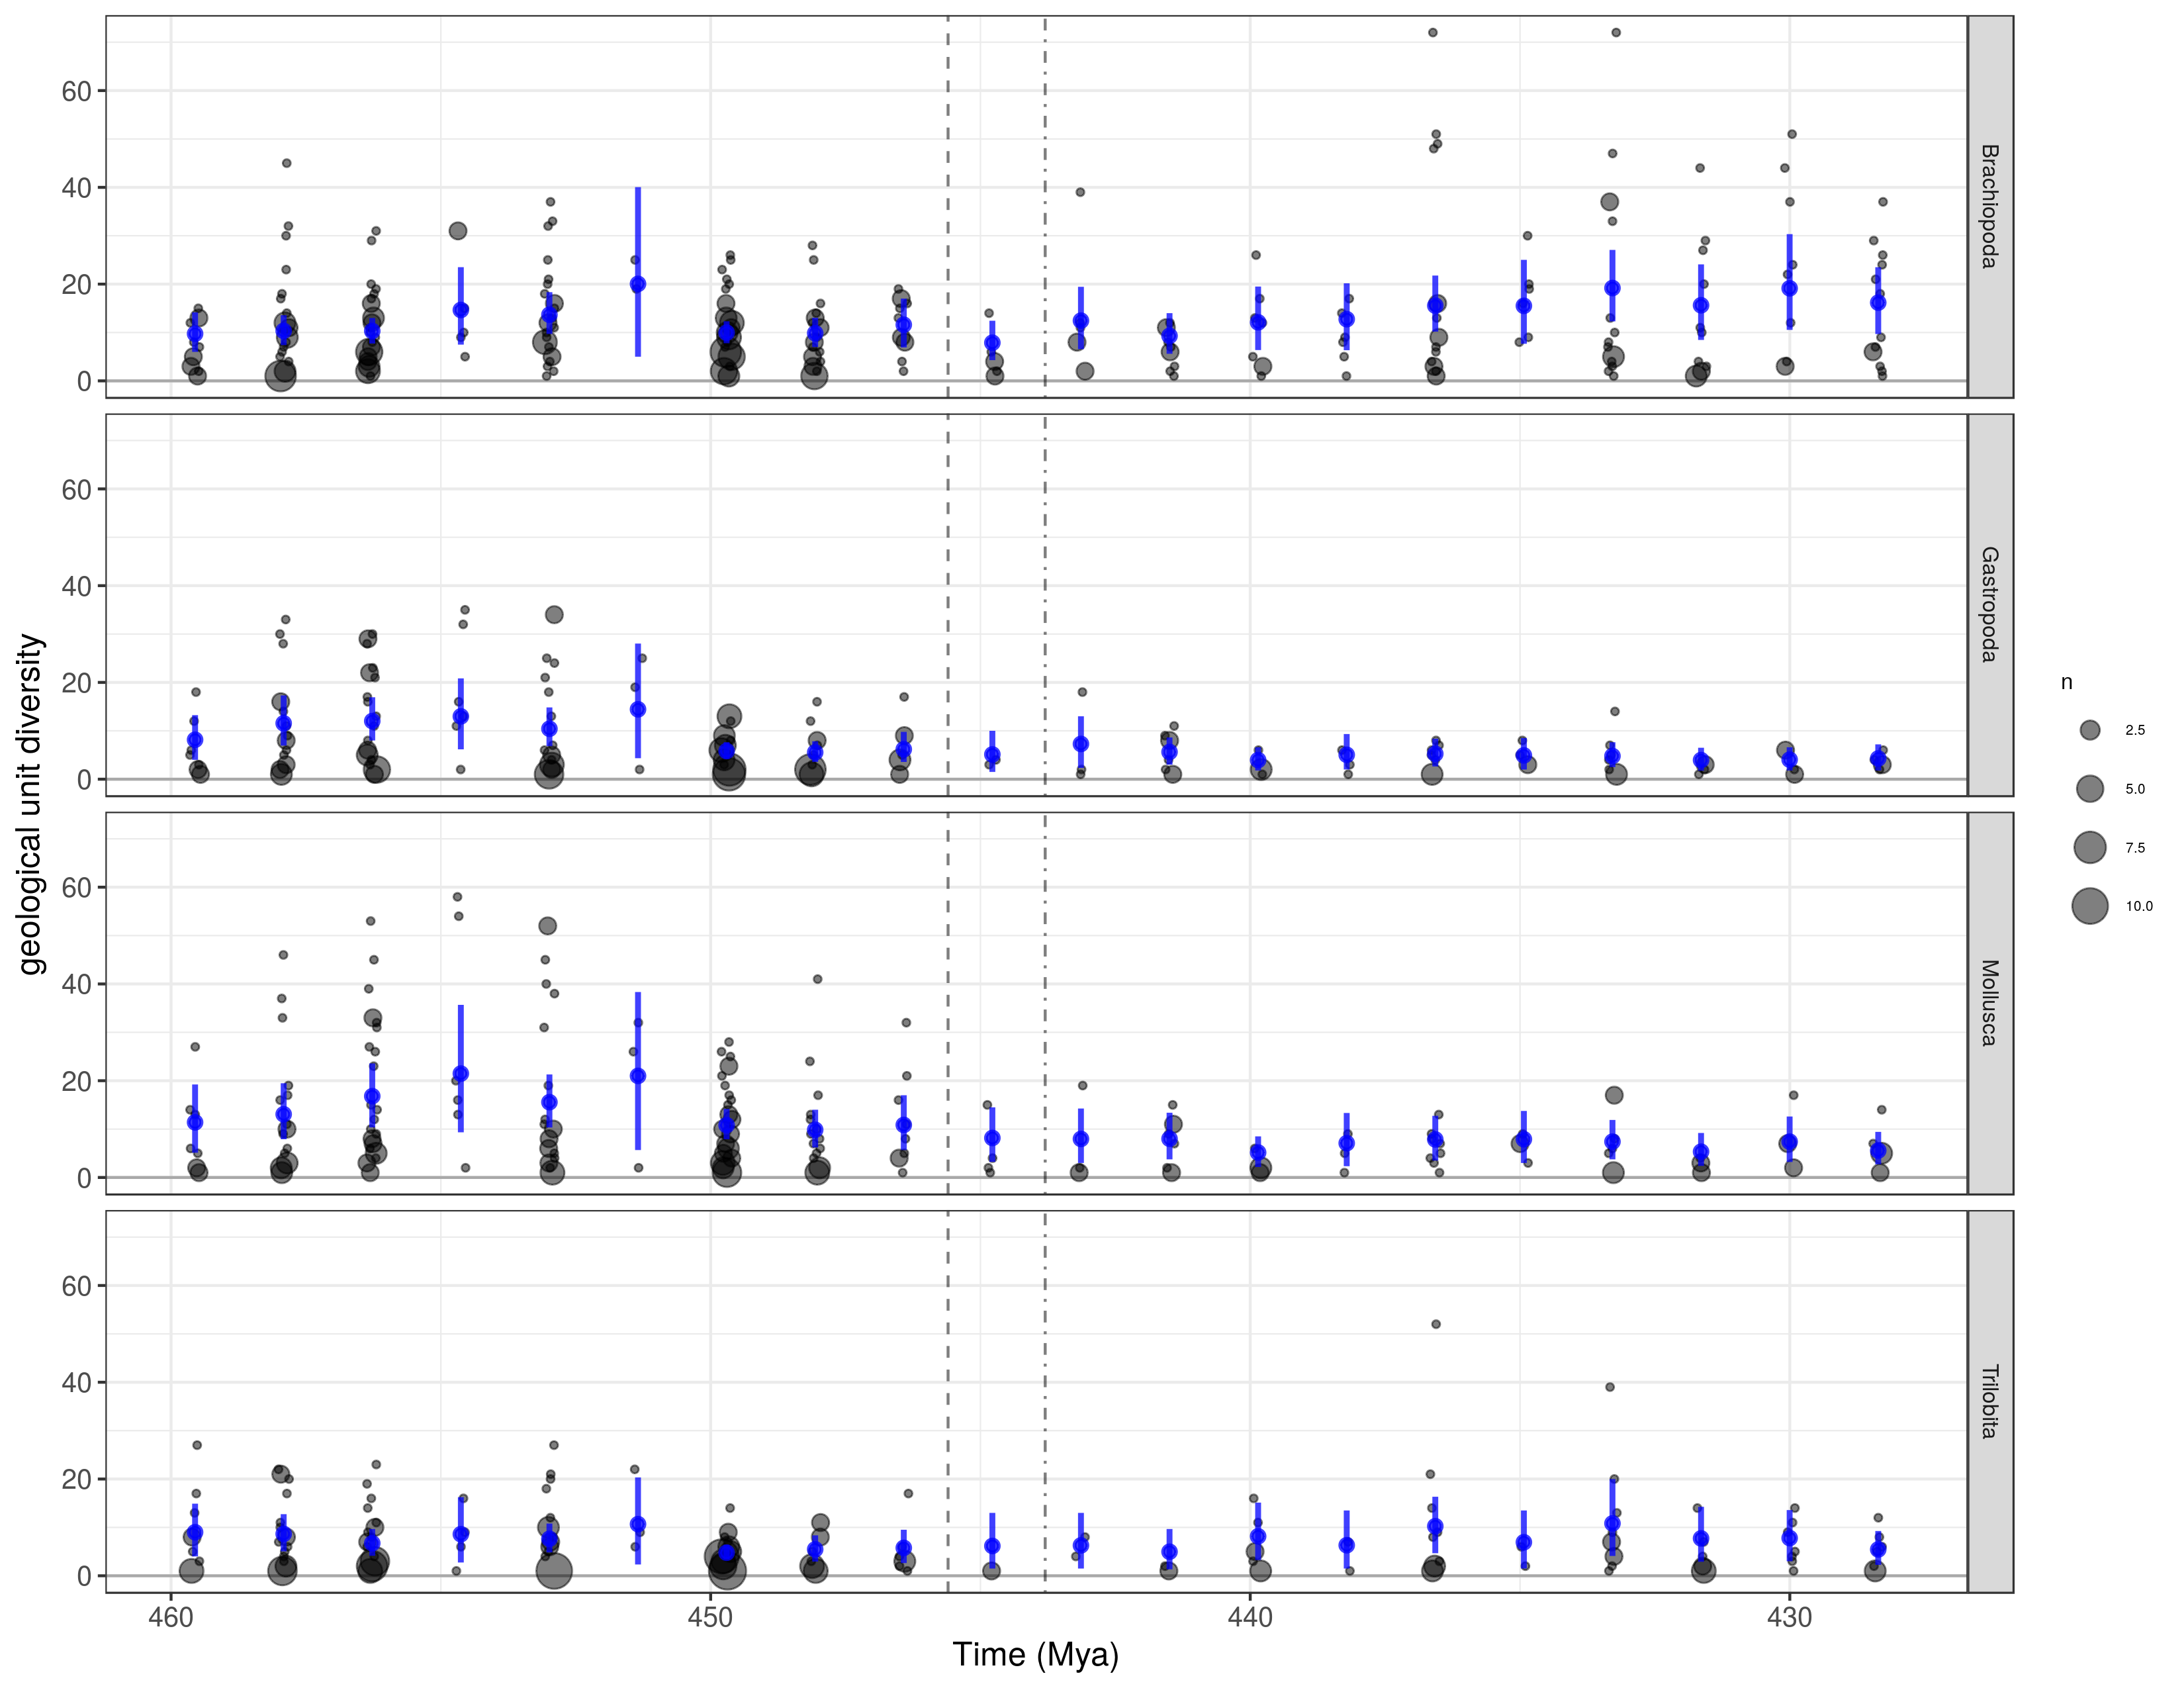
\includegraphics[width=\textwidth,height=0.5\textheight,keepaspectratio=true]{figure/unitdiv_time}
  \caption{<+caption text+>}
  \label{fig:<+label+>}
\end{figure}



\subsection{Effects of geological covariates on estimated diversity}
% what is the point of this section?
%   we've estimated the effect of multiple covariates
%   these estimates are allowed to vary through time
%     temporal structure is taken into account
%   what is the general relationship? what happens during hirnantian?
%     if all units have the same relationship
%       and all good bin estimates
%         there is no change in unit diversity though time
%         there is no change in geol properties that affect unit diversity
%       and some bad bin estimates
%         our model can not explain these bins; something is going on here
%     if some units have diff relationships (sign change, effect loss)
%       and all good bin estimates
%         we capture the changing relationship between preservational context and observed diversity
%       and some bad bin estimates
%         our model can not explain these bins; something is going on here


% time series graph
% what does this graph represent?
%   effect of covariate on expected count over time
%   violin shows full posterior estimate
%   pointrange shows mean with 80CI
\begin{figure}[ht]
  \centering
  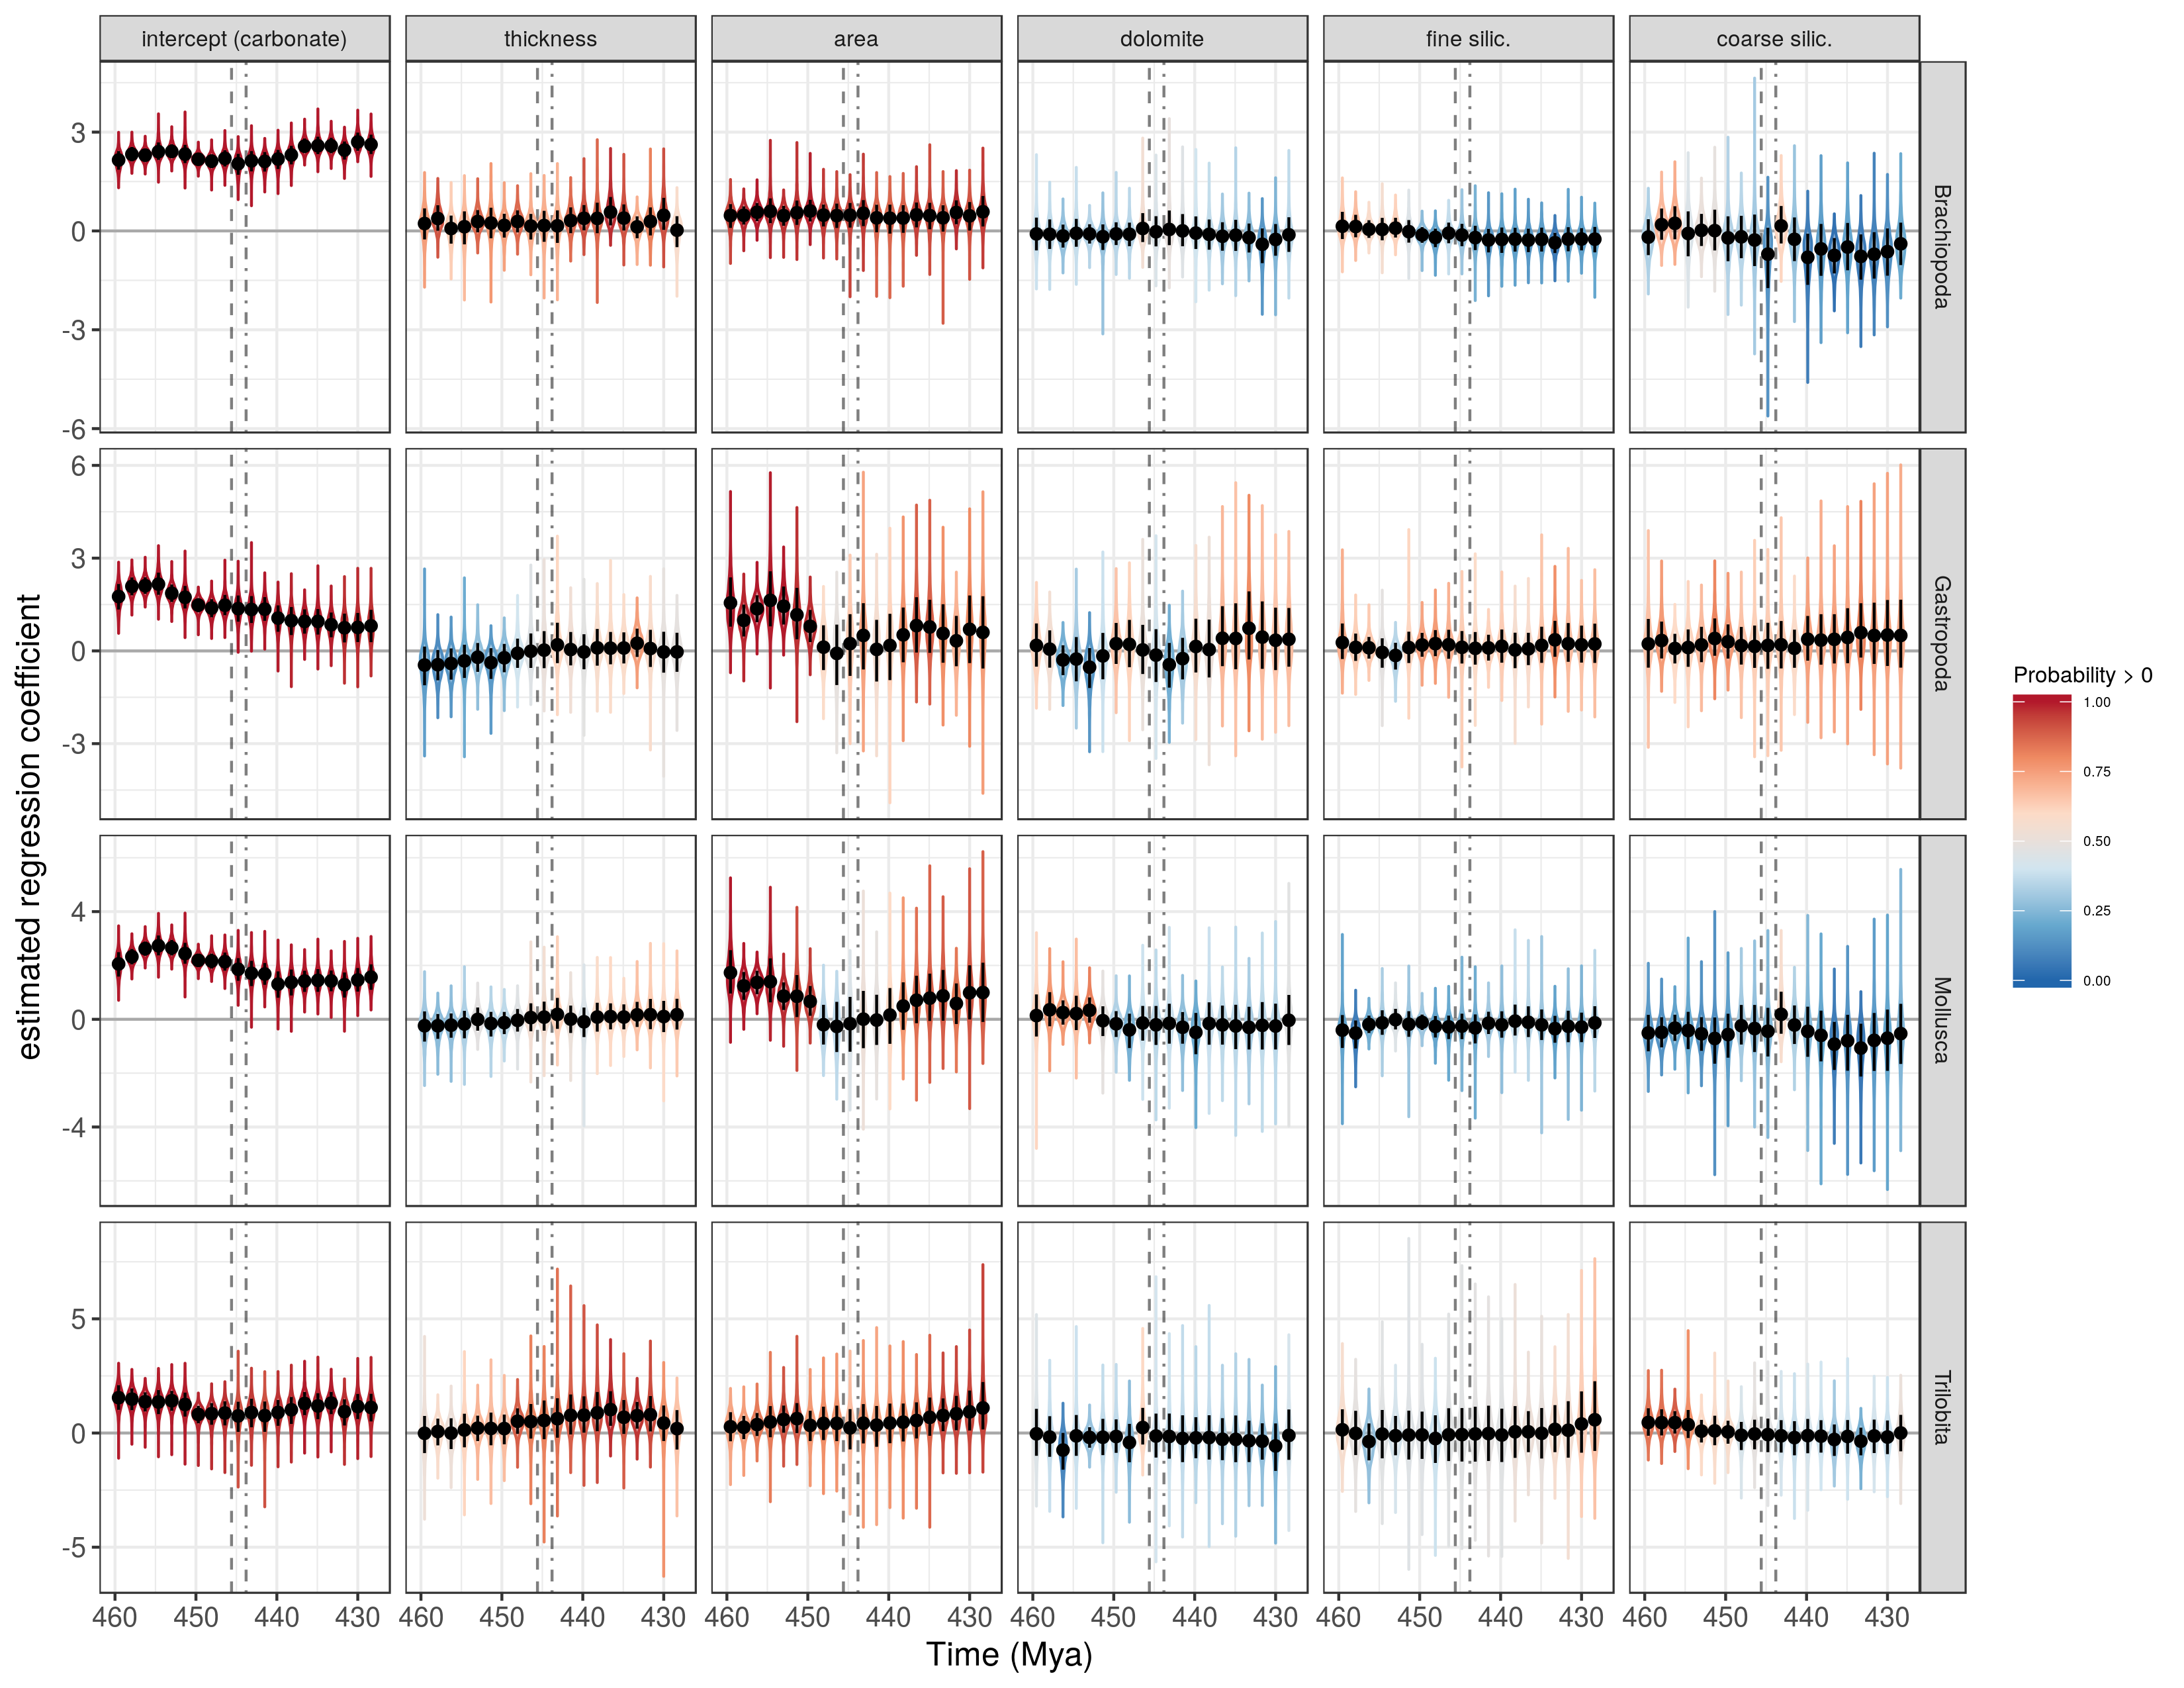
\includegraphics[width=\textwidth,height=0.5\textheight,keepaspectratio=true]{figure/cov_time}
  \caption{<+caption text+>}
  \label{fig:<+label+>}
\end{figure}

% covariance of effect change?
%   are effects correlated in their changes through time?



\end{document}
